\chapter{Existing molecular algorithms for {\sc Satisfiability}}

%<Paragraph> Introduce two molecular algorithms for {\sc Satisfiability}

In this chapter, we discuss two molecular algorithms for {\sc Satisfiability}.  These algorithms construct sets of all witnesses for {\sc Satisfiability} instances.  Lipton's algorithm requires a combinatorial space of all witness candidates to be constructed and then filters out invalid ones.  Ogihara and Ray's algorithm constructs a set of witness candidates throughout execution.  Following the description, we explore the physical implementations of---and simulation frameworks for---these algorithms.

\begin{table}[htdp]
\caption{Components of Boolean literals and equivalent literal representations.}
\begin{center}
\begin{tabular}{| c | c | c | c | c |}
\hline
\textbf{Literal} & \textbf{Variable} $(v)$ & \textbf{Polarity} $(P)$ & \textbf{DIMACS} $(\pm v)$ & \textbf{Condensed} $(v_P)$ \\ \hline	
$x_1$ & $1$ & $\texttt{T}$ & $1$ & $1_{\texttt{T}}$ \\
$\neg x_1$ & $1$ & $\texttt{F}$ & $-1$ & $1_{\texttt{F}}$ \\
$x_n$ & $n$ & $\texttt{T}$ & $n$ & $n_{\texttt{T}}$ \\
$\neg x_n$ & $n$ & $\texttt{F}$ & $-n$ & $n_{\texttt{F}}$ \\ \hline
\end{tabular}
\end{center}
\label{equivalentLiteralTable}
\end{table}%

The algorithm definitions and example traces use the literal conventions listed in Table \ref{equivalentLiteralTable}.  Table \ref{equivalentLiteralTable} lists components of a literal (variable and polarity), along with equivalent forms (DIMACS and a condensed representation).  

In Chapter 1, witness candidates for {\sc Satisfiability} were represented as a bit-vector $B$.  Consider the equivalent representation for witness candidates in Figure \ref{equivalentWitnessRepresentations}.

\begin{figure}[htbp]
\begin{center}

	\begin{align*}
	B &= [0, 1, 0, 1 \rangle \\
	L &= \{ \neg x_1, x_2, \neg x_3, x_4 \} \\
	D &= \texttt{SFTFT}\\ 
	Z &= \texttt{S-1+2-3+4}\\ 
	\end{align*}

\caption{The bit-vector $B = [0, 1, 0, 1 \rangle$ can be represented as the set of literal assignments $L = \{ \neg x_1, x_2, \neg x_3, x_4 \}$.  A directed polarity string (D) with initial sequence (\texttt{S}), followed by a sequence of literals provides $D = \texttt{SFTFT}$.  A directed integer string (Z) consists of an initial sequence (\texttt{S}) followed by DIMACS literal assignments $Z =\texttt{S-1+2-3+4}$. }
\label{equivalentWitnessRepresentations}
\end{center}
\end{figure}

\FloatBarrier

We use the directed string notation (representation $D$ in Figure \ref{equivalentWitnessRepresentations}) as shorthand for a directed oligonucleotide.  The directed string representation $D$ can be indexed by the variable $v$ using the condensed literal from Table \ref{equivalentLiteralTable}.  In Lipton's algorithm, literal configurations for a variable $v$ get extracted directly ($v_{\texttt{T}}$ or $v_{\texttt{F}}$).

Ogihara and Ray's algorithm extracts satisfying literal configurations from an ordered clause $(a, b, c)$.  We use the condensed literal notation $v_P$ to indicate the assignment (either \texttt{T} or \texttt{F}) for the literal $v$.  

In the discussion of the Distribution algorithm in Chapter 4, we use the directed integer notation (representation $Z$ in Figure \ref{equivalentWitnessRepresentations}) as shorthand for a directed sequence of integers.

Along with our shorthand representations ($D$ and $Z$) from Figure \ref{equivalentWitnessRepresentations}, we include a small combinatorial library corresponding to positive and negative literals.  Table \ref{smallCombinatorialLibrary} lists a mapping of literals to oligonucleotides used for literal matching and assignment.  


\begin{table}[htdp]
\caption{Positive and negative literal assignment and matching oligonucleotides.  }
\begin{center}
\begin{tabular}{|c|c|c|}
\hline
\textbf{Literal} & \textbf{Assignment} & \textbf{Matching} \\ \hline
$x_1$ & $5'-$\texttt{TTT}$-3'$ & $3'-$\texttt{AAA}$-5'$ \\ 
$\neg x_1$ & $5'-$\texttt{TTA}$-3'$ & $3'-$\texttt{AAT}$-5'$ \\ \hline
$x_2$ & $5'-$\texttt{CTT}$-3'$ & $3'-$\texttt{GAA}$-5'$ \\ 
$\neg x_2$ & $5'-$\texttt{ATT}$-3'$ & $3'-$\texttt{TAA}$-5'$ \\ \hline
$x_3$ & $5'-$\texttt{ATG}$-3'$ & $3'-$\texttt{TAC}$-5'$ \\ 
$\neg x_3$ & $5'-$\texttt{GTT}$-3'$ & $3'-$\texttt{CAA}$-5'$ \\ \hline
$x_4$ & $5'-$\texttt{TCT}$-3'$ & $3'-$\texttt{AGA}$-5'$ \\ 
$\neg x_4$ & $5'-$\texttt{CCT}$-3'$ & $3'-$\texttt{GGA}$-5'$ \\ \hline
$x_5$ & $5'-$\texttt{ACT}$-3'$ & $3'-$\texttt{TGA}$-5'$ \\ 
$\neg x_5$ & $5'-$\texttt{GCT}$-3'$ & $3'-$\texttt{CGA}$-5'$ \\ \hline
Start & $5'-$\texttt{TTG}$-3'$ & $3'-$\texttt{AAC}$-5'$ \\ \hline
\end{tabular}
\end{center}
\label{smallCombinatorialLibrary}
\end{table}%

\FloatBarrier

The examples throughout this report use this combinatorial library designed with codons.  Larger combinatorial libraries \cite{dnaComputingModels2008} take multiple considerations for the genetic encoding, including uniform melting temperature and non-self complementary sequences.  Codons provide redundant encodings that we exploit for a small library.   


\section{Lipton's algorithm for {\sc Satisfiability}}

%	<Paragraph> Introduce Lipton's algorithm

Introduced in 1995 by Richard Lipton \cite{Lipton95usingdna}, this algorithm filters satisfiable witnesses from a combinatorial space of all witness candidates.  Lipton's algorithm is analogous to a conventional brute-force search for all witnesses of a {\sc Satisfiability} instance.

Lipton's algorithm (Algorithm \ref{liptonAlgorithm}) first constructs a combinatorial space $T$ containing oligonucleotide configurations for all potential witness candidates.  The algorithm iterates over each of the clauses $C$ in $\phi$.  

From each clause $C$, each of the literals contained within each clause $C$ get filtered to satisfiable witnesses.  The contents of $T$ get filtered by incrementally extracting those literals that satisfy the current clause.  The next iteration filters witnesses that satisfy the previous clauses from $T$ and the literal contents from $C$.  The algorithm terminates with a set of witnesses $T$ for the CNF input $\phi$.  If $\phi$ is unsatisfiable, then $T = \emptyset$.  

% We iterate over each of the clauses in $\phi$.  Each clause iteration filters the contents of the tube $T$ to only witnesses that satisfy the current clause.  

	
\begin{figure}[htbp]
\begin{center}
	\begin{pseudocode}{Lipton's Algorithm}{\phi}
	T \GETS \text{{\sc Combinatorial Generate}}(n) \\
	\FOREACH \text{clause } C \text{ in } \phi \DO
		\BEGIN
		T_c \GETS \emptyset \\
		\FOREACH \text{literal } v \text{ in } C \DO
			\BEGIN
				\IF v \text{ is a positive literal} \THEN
					\BEGIN
						T_P \GETS \text{extract}(T, v_{\texttt{T}})\\
						T_c \GETS \text{mix}(T_P, T_c)						
					\END
				\ELSE
					\BEGIN
						T_N \GETS \text{extract}(T, v_{\texttt{F}})\\
						T_c \GETS \text{mix}(T_N, T_c)						
					\END
			\END
		\\
		T \GETS \text{purify(}T_c\text{)} \\
		\END
	\\
	\RETURN{\text{detect}(T)}
	\end{pseudocode}

\caption{{\sc Lipton's Algorithm} iterates over each of the $m$ clauses.  The contents of $T_C$ grows incrementally with configurations from $T$ that satisfy the literal $v$.  Once the entire clause $C$ has been evaluated, $T_C$ contains configurations that witness the observed conditions.  The contents of $T_C$ are stored as $T$ for the next clause; $T$ now contains configurations that witness all previous clauses.  Once complete, the tube $T$ contains all witnesses for $\phi$, if any witnesses exist.}
\label{liptonAlgorithm}
\end{center}
\end{figure}


\FloatBarrier

	\subsection{Description of Lipton's algorithm}
		
%		<Paragraph> Describe setup
The function {\sc Combinatorial Generate} (Algorithm \ref{combinatorialGenerate}) implements the split-mix synthesis technique \cite{furka1982, furkaBook}.  {\sc Combinatorial Generate} returns a tube $T_{comb}$ consisting of oligonucleotides that represent all $2^n$ distinct witness candidates.  The tube $T_{comb}$ begins with an initial medium denoted by \texttt{S}.  An iterative loop extends $T_{comb}$ using split-mix synthesis.  Each split corresponds with appending the tubes with a true (\texttt{T}) and false (\texttt{F}) assignment.  The two tubes are mixed and purified to contain equimolar portions of each witness candidate.  




\begin{figure}[htbp]
\begin{center}

	\begin{pseudocode}{Combinatorial Generate}{n}
		T_{comb} \GETS \emptyset \\
		T_{comb} \GETS \text{mix(}T_{comb}, \texttt{S} \text{)} \\ 
	
		\FOR v \GETS 1 \text{ to } n \DO
			\BEGIN
			
			[T_1,T_2] \GETS \text{split(} T_{comb}\text{)}\\
			T_1 \GETS \text{append(}T_1, v_{\texttt{T}} \text{)}\\
			T_2 \GETS \text{append(}T_2, v_{\texttt{F}} \text{)}\\
			T_{comb} \GETS \text{mix(}T_1,T_2\text{)}\\
		\END
		\\
		\RETURN {T_{comb}}
	\end{pseudocode}

\caption{{\sc Combinatorial Generate} constructs a combinatorial space consisting of $2^n$ molecular configurations in polynomial time.}
\label{combinatorialGenerate}
\end{center}
\end{figure}

\FloatBarrier

Let us consider an example execution of {\sc Combinatorial Generate} with $n = 2$.

\noindent The tube $T_{comb}$ begins as an empty tube.  A start configuration \texttt{S} initiates the tube $T_{comb}$ with a medium for combinatorial synthesis.

\noindent We begin with the initial contents

\begin{center}
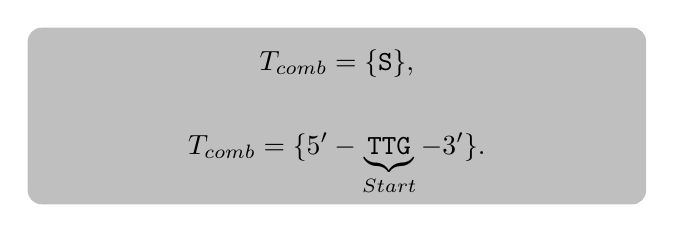
\begin{tikzpicture}
\node[fill=lightgray, rounded corners=5pt, text width=3in]{
\[
T_{comb} = \{ \texttt{S} \},
\]

\[
T_{comb} = \{ 5'-\underbrace{\texttt{TTG}}_{\text{Start}}-3' \}.
\]
};
\end{tikzpicture}
\end{center}

\noindent Iteration $v = 1$:

First, split the contents of $T_{comb}$.  We have

\begin{center}
\begin{tikzpicture}
\node[fill=gray, rounded corners=5pt, text width=6in]{

	\makebox[\textwidth][r]{
		\begin{minipage}[t]{0.5\textwidth}
			\begin{center}
			\begin{tikzpicture}
			\node[fill=lightgray, rounded corners=5pt, text width=2.5in]{
				\[
					T_1 = \{ \texttt{S} \}
				\]
				\[
					T_1 = \{ 5'-\underbrace{\texttt{TTG}}_{\text{Start}}-3' \}
				\]
			};
			\end{tikzpicture}
			\end{center}
		\end{minipage}				
		\begin{minipage}[t]{0.5\textwidth}
			\begin{center}
			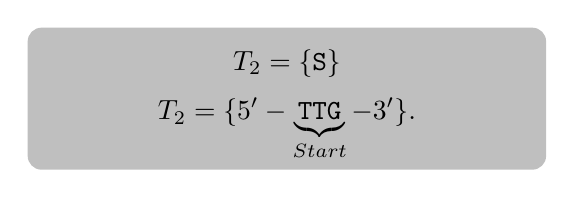
\begin{tikzpicture}
			\node[fill=lightgray, rounded corners=5pt, text width=2.5in]{
				\[
					T_2 = \{ \texttt{S} \}
				\]
				\[
					T_2 = \{ 5'-\underbrace{\texttt{TTG}}_{\text{Start}}-3' \}.
				\]
			};
			\end{tikzpicture}
			\end{center}
		\end{minipage}		
	}
};
\end{tikzpicture}
\end{center}
\hspace{1em}

Next, append each of the tubes with a positive (\texttt{T}) and negative (\texttt{F}) assignment for the literal $v_1$.  We have

\begin{center}
\begin{tikzpicture}
\node[fill=gray, rounded corners=5pt, text width=6in]{
	\makebox[\textwidth][r]{
		\begin{minipage}[t]{0.5\textwidth}
			\begin{center}
			\begin{tikzpicture}
			\node[fill=lightgray, rounded corners=5pt, text width=2.5in]{
				\[
					T_1 = \{ \texttt{ST} \}
				\]
				\[
					T_1 = \{ 5'-\underbrace{\texttt{TTG}}_{\text{Start}}\cdot\underbrace{\texttt{TTT}}_{ x_{1}}-3' \}
				\]
			};
			\end{tikzpicture}
			\end{center}			
		\end{minipage}				
		\begin{minipage}[t]{0.5\textwidth}
			\begin{center}
			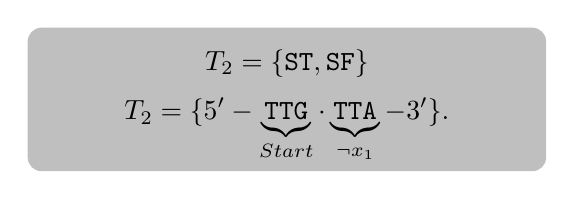
\begin{tikzpicture}
			\node[fill=lightgray, rounded corners=5pt, text width=2.5in]{			
				\[
					T_2 = \{\texttt{ST}, \texttt{SF}\}
				\]
				\[
					T_2 = \{ 5'-\underbrace{\texttt{TTG}}_{\text{Start}}\cdot\underbrace{\texttt{TTA}}_{\neg x_{1}}-3' \}.		
				\]
			};
			\end{tikzpicture}
			\end{center}		
		\end{minipage}		
	}
};
\end{tikzpicture}
\end{center}

\hspace{1em}

Mix the contents of $T_1$ and $T_2$ to form $T_{comb}$ for the next iteration.  We have

\begin{center}
\begin{tikzpicture}
\node[fill=lightgray, rounded corners=5pt, text width=3in]{
\[
T_{comb} = \{\texttt{ST}, \texttt{SF}\}.
\]
\begin{align*}
T_{comb} = \{&5'-\underbrace{\texttt{TTG}}_{\text{Start}}\cdot\underbrace{\texttt{TTT}}_{ x_{1}}-3',\\
&5'-\underbrace{\texttt{TTG}}_{\text{Start}}\cdot\underbrace{\texttt{TTA}}_{\neg x_{1}}-3' \}.
\end{align*}
};
\end{tikzpicture}
\end{center}

\noindent Iteration $v = 2$:

Split the contents of $T_{comb}$.  We have

\begin{center}
\begin{tikzpicture}
\node[fill=gray, rounded corners=5pt, text width=6in]{
	\makebox[\textwidth][l]{
		\begin{minipage}[t]{0.5\textwidth}
			\begin{center}
			\begin{tikzpicture}
			\node[fill=lightgray, rounded corners=5pt, text width=2.5in]{		
				\[
				T_1 = \{\texttt{ST}, \texttt{SF}\}
				\]
				\begin{align*}
				T_{1} = \{&5'-\underbrace{\texttt{TTG}}_{\text{Start}}\cdot\underbrace{\texttt{TTT}}_{ x_{1}}-3',\\
						  &5'-\underbrace{\texttt{TTG}}_{\text{Start}}\cdot\underbrace{\texttt{TTA}}_{\neg x_{1}}-3' \}
				\end{align*}
			};
			\end{tikzpicture}
			\end{center}				
		\end{minipage}				
		\begin{minipage}[t]{0.5\textwidth}
			\begin{center}
			\begin{tikzpicture}
			\node[fill=lightgray, rounded corners=5pt, text width=2.5in]{
				\[
				 T_2 = \{\texttt{ST}, \texttt{SF}\}
				\]
				\begin{align*}	
				T_{2} = \{&5'-\underbrace{\texttt{TTG}}_{\text{Start}}\cdot\underbrace{\texttt{TTT}}_{ x_{1}}-3',\\
						  &5'-\underbrace{\texttt{TTG}}_{\text{Start}}\cdot\underbrace{\texttt{TTA}}_{\neg x_{1}}-3' \}.
				\end{align*}
			};
			\end{tikzpicture}
			\end{center}				
		\end{minipage}		
	}
};
\end{tikzpicture}
\end{center}
	
\hspace{1em}

Next, append each of the tubes with a positive (\texttt{T}) and negative (\texttt{F}) assignment for the literal $v_2$.  We have

\begin{center}
\begin{tikzpicture}
\node[fill=gray, rounded corners=5pt, text width=6in]{
	\makebox[\textwidth][r]{
		\begin{minipage}[t]{0.5\textwidth}
			\begin{center}
			\begin{tikzpicture}
			\node[fill=lightgray, rounded corners=5pt, text width=2.5in]{		
				\[
				T_1 = \{\texttt{STT}, \texttt{SFT}\}
				\]
				\begin{align*}
				T_{1} = \{&5'-\underbrace{\texttt{TTG}}_{\text{Start}}\cdot\underbrace{\texttt{TTT}}_{ x_{1}}\cdot\underbrace{\texttt{CTT}}_{ x_{2}}-3',\\
						  &5'-\underbrace{\texttt{TTG}}_{\text{Start}}\cdot\underbrace{\texttt{TTA}}_{\neg x_{1}}\cdot\underbrace{\texttt{CTT}}_{ x_{2}}-3' \}
				\end{align*}
			};
			\end{tikzpicture}
			\end{center}				
		\end{minipage}				
		\begin{minipage}[t]{0.5\textwidth}
			\begin{center}
			\begin{tikzpicture}
			\node[fill=lightgray, rounded corners=5pt, text width=2.5in]{
				\[
				T_2 = \{\texttt{STF}, \texttt{SFF}\}		
				\]
				\begin{align*}	
				T_{2} = \{&5'-\underbrace{\texttt{TTG}}_{\text{Start}}\cdot\underbrace{\texttt{TTT}}_{ x_{1}}\cdot\underbrace{\texttt{ATT}}_{\neg x_{2}}-3',\\
						  &5'-\underbrace{\texttt{TTG}}_{\text{Start}}\cdot\underbrace{\texttt{TTA}}_{\neg x_{1}}\cdot\underbrace{\texttt{ATT}}_{\neg x_{2}}-3' \}.
				\end{align*}
			};
			\end{tikzpicture}
			\end{center}				
		\end{minipage}		
	}
};
\end{tikzpicture}
\end{center}
\hspace{1em}

Mix the contents of $T_1$ and $T_2$ to form $T_{comb}$ for the final iteration.  The algorithm {\sc Combinatorial Generate} returns the following tube

\begin{center}
\begin{tikzpicture}
\node[fill=lightgray, rounded corners=5pt, text width=3in]{
	\[
	T_{comb} = \{\texttt{STT}, \texttt{SFT}, \texttt{STF}, \texttt{SFF}\},
	\]
	\begin{align*}
	T_{comb} = \{&5'-\underbrace{\texttt{TTG}}_{\text{Start}}\cdot\underbrace{\texttt{TTT}}_{ x_{1}}\cdot\underbrace{\texttt{CTT}}_{ x_{2}}-3',\\
			  &5'-\underbrace{\texttt{TTG}}_{\text{Start}}\cdot\underbrace{\texttt{TTA}}_{\neg x_{1}}\cdot\underbrace{\texttt{CTT}}_{ x_{2}}-3',\\
			  &5'-\underbrace{\texttt{TTG}}_{\text{Start}}\cdot\underbrace{\texttt{TTT}}_{ x_{1}}\cdot\underbrace{\texttt{ATT}}_{\neg x_{2}}-3',\\
			  &5'-\underbrace{\texttt{TTG}}_{\text{Start}}\cdot\underbrace{\texttt{TTA}}_{\neg x_{1}}\cdot\underbrace{\texttt{ATT}}_{\neg x_{2}}-3' \}.
	\end{align*}
};
\end{tikzpicture}
\end{center}	
%%%%%%%%%%%%%%%%%

{\sc Combinatorial Generate} generates all witness candidates for a {\sc Satisfiability} instance.  Lipton's algorithm filters, from a combinatorial space $T$, configurations that represent witnesses for the input $\phi$.

	\subsection{Detailed trace of Lipton's algorithm}	
%	<Paragraph> Introduce pseudocode
Appendix B lists a detailed execution trace for Lipton's algorithm.

%%%%%%%%%%%%%%%%%%%%%%%%%%%%%%%%%

\section{Ogihara and Ray's algorithm for {\sc Satisfiability}}

%	<Paragraph> Introduce Ogihara and Ray's algorithm

Ogihara and Ray's algorithm (Algorithm \ref{ogiharaRayAlgorithm}) consist of a breadth-first evaluation of clauses from a CNF formula \cite{Ogihara:1996:BFS:898228,Ogihara97dna-basedparallel}.  The algorithm constructs a set of witness candidates based on a parse of a 3-CNF formula.  In this section, we describe the preconditions and execution of Ogihara and Ray's algorithm.

%		<Paragraph> Describe execution

\begin{figure}[htbp]
	\renewcommand{\figurename}{Algorithm}
	\renewcommand{\thepseudocode}{\ref{ogiharaRayAlgorithm}}
	
	\begin{center}

	\begin{pseudocode}[shadowbox]{Ogihara and Ray's Algorithm}{\phi}
	
	\text{// Input $\phi$ consists of $n$ variables.}\\
	\text{// Each clause $C$ contains ordered literals $(a,b,c)$.}\\
	\text{// Extract literals using the condensed notation $v_P$, where: }\\
	\text{// \hspace{1em} $v_P$ matches the literal, and $v_N$ matches the negated literal.}\\
	\\
	T \GETS \{ \texttt{STT}, \texttt{STF}, \texttt{SFT},  \texttt{SFF}\} \\
	
	\FOR v \GETS 3 \text{ to } n \DO
		\BEGIN
		[T_P, T_N] \GETS \text{split}(T)\\
	
		\FOREACH \text{clause } C \text{ in } \phi \DO
			\BEGIN
				(a, b, c) \GETS C\\
				\IF v_{\texttt{T}} = c  \THEN
					\BEGIN
						T_{P1} \GETS \text{extract}(T_N, a_P)\\
						T_{N1} \GETS \text{extract}(T_N, a_N)\\				
						T_{P2} \GETS \text{extract}(T_{N1}, b_P)\\
						T_{N} \GETS \text{mix}(T_{P1}, T_{P2})\\
						T_{N} \GETS \text{purify(}T_{N}\text{)}					
					\END \\  
				\IF v_{\texttt{F}} = c \THEN
					\BEGIN
						T_{P1} \GETS \text{extract}(T_P, a_P)\\
						T_{N1} \GETS \text{extract}(T_P, a_N)\\				
						T_{P2} \GETS \text{extract}(T_{N1}, b_P)\\
						T_{P} \GETS \text{mix}(T_{P1}, T_{P2})\\
						T_{P} \GETS \text{purify(}T_{P}\text{)} 						
					\END\\
			\END\\
			T_P \GETS \text{append}(T_P, v_{\texttt{T}})\\
			T_N \GETS \text{append}(T_N, v_{\texttt{F}})\\
			T \GETS \text{mix}(T_P, T_N)\\
			T \GETS \text{purify(}T\text{)} \\									
		\END\\
	\RETURN{\text{detect}(T)}
	\end{pseudocode}

\caption{{\sc Ogihara and Ray's Algorithm} evaluates each subsequent variable and determines possible assignments.  The possible assignments for the variables $a$ and $b$ get extracted if $c$ matches the current variable $v$.  Effectively pruning only potential solutions.  These potential solutions $T_P$ and $T_N$ get appended with the positive or negative string assignments.  The algorithm continues until each variable gets evaluated.  The remaining space $T$ contains all solutions for the CNF instance $\phi$ after the algorithm terminates.}
\label{ogiharaRayAlgorithm}
\end{center}
\end{figure}

\FloatBarrier

\subsection{Description of Ogihara and Ray's algorithm}
		
Ogihara and Ray's algorithm begins with four initial witness candidates, we have

\begin{center}
\begin{tikzpicture}
\node[fill=lightgray, rounded corners=5pt, text width=3in]{
	\[
	T = \{ \texttt{STT}, \texttt{STF}, \texttt{SFT}, \texttt{SFF}\}
	\]
	\begin{align*}
	T = \{ &5'-\underbrace{\texttt{TTG}}_{\text{Start}}\cdot\underbrace{\texttt{TTT}}_{ x_{1}}\cdot\underbrace{\texttt{CTT}}_{ x_{2}}-3',\\
		   &5'-\underbrace{\texttt{TTG}}_{\text{Start}}\cdot\underbrace{\texttt{TTT}}_{ x_{1}}\cdot\underbrace{\texttt{ATT}}_{\neg x_{2}}-3',\\
		   &5'-\underbrace{\texttt{TTG}}_{\text{Start}}\cdot\underbrace{\texttt{TTA}}_{\neg x_{1}}\cdot\underbrace{\texttt{CTT}}_{ x_{2}}-3',\\
		   &5'-\underbrace{\texttt{TTG}}_{\text{Start}}\cdot\underbrace{\texttt{TTA}}_{\neg x_{1}}\cdot\underbrace{\texttt{ATT}}_{\neg x_{2}}-3'\}.
	\end{align*}
};
\end{tikzpicture}
\end{center}

For each clause $C = (x_i \vee x_j \vee x_k)$, we have that $1 \leq i < j < k \leq n$.  As an example, let us evaluate the clause
\[
C = x_1 \vee \neg x_2 \vee \neg x_3.
\]

\noindent On the first iteration, we compare the third ordered literal $c$ with $x_3$.  Since $c = \neg x_3$, extract configurations that satisfy $a \vee b$.  

\begin{center}
\begin{tikzpicture}
\node[fill=gray, rounded corners=5pt, text width=6in]{
	\makebox[\textwidth][r]{
		\begin{minipage}[t]{0.5\textwidth}
			\begin{center}
			\begin{tikzpicture}
			\node[fill=lightgray, rounded corners=5pt, text width=2.5in]{		
				\[
				T_P = \{ \texttt{STT}, \texttt{STF}, \texttt{SFT}, \texttt{SFF}\}
				\]
				\begin{align*}
				T_P = \{ &5'-\underbrace{\texttt{TTG}}_{\text{Start}}\cdot\underbrace{\texttt{TTT}}_{ x_{1}}\cdot\underbrace{\texttt{CTT}}_{ x_{2}}-3',\\
					   &5'-\underbrace{\texttt{TTG}}_{\text{Start}}\cdot\underbrace{\texttt{TTT}}_{ x_{1}}\cdot\underbrace{\texttt{ATT}}_{\neg x_{2}}-3',\\
					   &5'-\underbrace{\texttt{TTG}}_{\text{Start}}\cdot\underbrace{\texttt{TTA}}_{\neg x_{1}}\cdot\underbrace{\texttt{CTT}}_{ x_{2}}-3',\\
					   &5'-\underbrace{\texttt{TTG}}_{\text{Start}}\cdot\underbrace{\texttt{TTA}}_{\neg x_{1}}\cdot\underbrace{\texttt{ATT}}_{\neg x_{2}}-3'\},
				\end{align*}
			};
			\end{tikzpicture}
			\end{center}				
		\end{minipage}				
		\begin{minipage}[t]{0.5\textwidth}
			\begin{center}
			\begin{tikzpicture}
			\node[fill=lightgray, rounded corners=5pt, text width=2.5in]{
				\[
				T_N = \{ \texttt{STT}, \texttt{STF}, \texttt{SFT}, \texttt{SFF}\}		
				\]
				\begin{align*}	
				T_N = \{ &5'-\underbrace{\texttt{TTG}}_{\text{Start}}\cdot\underbrace{\texttt{TTT}}_{ x_{1}}\cdot\underbrace{\texttt{CTT}}_{ x_{2}}-3',\\
					   &5'-\underbrace{\texttt{TTG}}_{\text{Start}}\cdot\underbrace{\texttt{TTT}}_{ x_{1}}\cdot\underbrace{\texttt{ATT}}_{\neg x_{2}}-3',\\
					   &5'-\underbrace{\texttt{TTG}}_{\text{Start}}\cdot\underbrace{\texttt{TTA}}_{\neg x_{1}}\cdot\underbrace{\texttt{CTT}}_{ x_{2}}-3',\\
					   &5'-\underbrace{\texttt{TTG}}_{\text{Start}}\cdot\underbrace{\texttt{TTA}}_{\neg x_{1}}\cdot\underbrace{\texttt{ATT}}_{\neg x_{2}}-3'\}.
				\end{align*}
			};
			\end{tikzpicture}
			\end{center}				
		\end{minipage}		
	}
};
\end{tikzpicture}
\end{center}
	
\hspace{1em}

\noindent From $T$, select configurations that satisfy $a = a_{\texttt{T}}$

\begin{center}
\begin{tikzpicture}
\node[fill=lightgray, rounded corners=5pt, text width=3in]{
	\[
	T_{P1} = \{ \texttt{STT}, \texttt{STF} \}.
	\]
	\begin{align*}
	T_{P1} = \{ &5'-\underbrace{\texttt{TTG}}_{\text{Start}}\cdot\underbrace{\texttt{TTT}}_{ x_{1}}\cdot\underbrace{\texttt{CTT}}_{ x_{2}}-3', \\
				&5'-\underbrace{\texttt{TTG}}_{\text{Start}}\cdot\underbrace{\texttt{TTT}}_{ x_{1}}\cdot\underbrace{\texttt{ATT}}_{\neg x_{2}}-3'\}
	\end{align*}
};
\end{tikzpicture}
\end{center}

\noindent From $T$, Select configurations that satisfy $\neg a = a_{\texttt{F}}$

\begin{center}
\begin{tikzpicture}
\node[fill=lightgray, rounded corners=5pt, text width=3in]{
	\[
	T_{N1} = \{ \texttt{SFT}, \texttt{SFF} \}.
	\]
	\begin{align*}
	T_{N1} = \{ &5'-\underbrace{\texttt{TTG}}_{\text{Start}}\cdot\underbrace{\texttt{TTA}}_{\neg x_{1}}\cdot\underbrace{\texttt{CTT}}_{ x_{2}}-3',\\
				&5'-\underbrace{\texttt{TTG}}_{\text{Start}}\cdot\underbrace{\texttt{TTA}}_{\neg x_{1}}\cdot\underbrace{\texttt{ATT}}_{\neg x_{2}}-3'\}
	\end{align*}
};
\end{tikzpicture}
\end{center}

\noindent From $T_{N1}$, select configurations that satisfy $b = b_{\texttt{F}}$
\begin{center}
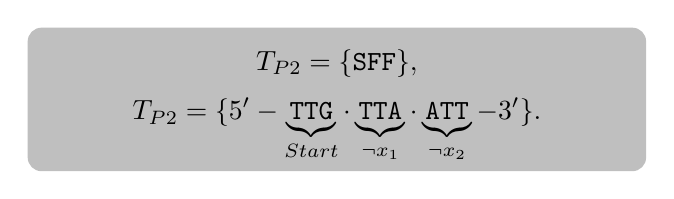
\begin{tikzpicture}
\node[fill=lightgray, rounded corners=5pt, text width=3in]{
	\[
	T_{P2} = \{ \texttt{SFF} \},
	\]
	\[
	T_{P2} = \{ 5'-\underbrace{\texttt{TTG}}_{\text{Start}}\cdot\underbrace{\texttt{TTA}}_{\neg x_{1}}\cdot\underbrace{\texttt{ATT}}_{\neg x_{2}}-3'\}.
	\]
};
\end{tikzpicture}
\end{center}

\noindent Mix the contents of $T_{P1}$ and $T_{P2}$ as the contents of $T_P$

\begin{center}
\begin{tikzpicture}
\node[fill=lightgray, rounded corners=5pt, text width=3in]{
	\[
	T_P = \{ \texttt{STT}, \texttt{STF}, \texttt{SFF} \},
	\]
	\begin{align*}
	T_P = \{ &5'-\underbrace{\texttt{TTG}}_{\text{Start}}\cdot\underbrace{\texttt{TTT}}_{ x_{1}}\cdot\underbrace{\texttt{CTT}}_{ x_{2}}-3', \\
			 &5'-\underbrace{\texttt{TTG}}_{\text{Start}}\cdot\underbrace{\texttt{TTT}}_{ x_{1}}\cdot\underbrace{\texttt{ATT}}_{\neg x_{2}}-3', \\
			 &5'-\underbrace{\texttt{TTG}}_{\text{Start}}\cdot\underbrace{\texttt{TTA}}_{\neg x_{1}}\cdot\underbrace{\texttt{ATT}}_{\neg x_{2}}-3'\}.
	\end{align*}
};
\end{tikzpicture}
\end{center}

\noindent We have the tubes

\begin{center}
\begin{tikzpicture}
\node[fill=gray, rounded corners=5pt, text width=6in]{
	\makebox[\textwidth][r]{
		\begin{minipage}[t]{0.5\textwidth}
			\begin{center}
			\begin{tikzpicture}
			\node[fill=lightgray, rounded corners=5pt, text width=2.5in]{		
				\[
				T_P = \{ \texttt{STT}, \texttt{STF}, \texttt{SFF} \}
				\]
				\begin{align*}
				T_P = \{ &5'-\underbrace{\texttt{TTG}}_{\text{Start}}\cdot\underbrace{\texttt{TTT}}_{ x_{1}}\cdot\underbrace{\texttt{CTT}}_{ x_{2}}-3', \\
						 &5'-\underbrace{\texttt{TTG}}_{\text{Start}}\cdot\underbrace{\texttt{TTT}}_{ x_{1}}\cdot\underbrace{\texttt{ATT}}_{\neg x_{2}}-3', \\
						 &5'-\underbrace{\texttt{TTG}}_{\text{Start}}\cdot\underbrace{\texttt{TTA}}_{\neg x_{1}}\cdot\underbrace{\texttt{ATT}}_{\neg x_{2}}-3'\},\\
				\end{align*}
			};
			\end{tikzpicture}
			\end{center}				
		\end{minipage}		
		\begin{minipage}[t]{0.5\textwidth}
			\begin{center}
			\begin{tikzpicture}
			\node[fill=lightgray, rounded corners=5pt, text width=2.5in]{		
				\[
				T_N = \{ \texttt{STT}, \texttt{STF}, \texttt{SFT}, \texttt{SFF}\}
				\]
				\begin{align*}
				T_N = \{ &5'-\underbrace{\texttt{TTG}}_{\text{Start}}\cdot\underbrace{\texttt{TTT}}_{ x_{1}}\cdot\underbrace{\texttt{CTT}}_{ x_{2}}-3',\\
					   &5'-\underbrace{\texttt{TTG}}_{\text{Start}}\cdot\underbrace{\texttt{TTT}}_{ x_{1}}\cdot\underbrace{\texttt{ATT}}_{\neg x_{2}}-3',\\
					   &5'-\underbrace{\texttt{TTG}}_{\text{Start}}\cdot\underbrace{\texttt{TTA}}_{\neg x_{1}}\cdot\underbrace{\texttt{CTT}}_{ x_{2}}-3',\\
					   &5'-\underbrace{\texttt{TTG}}_{\text{Start}}\cdot\underbrace{\texttt{TTA}}_{\neg x_{1}}\cdot\underbrace{\texttt{ATT}}_{\neg x_{2}}-3'\}.
				\end{align*}
			};
			\end{tikzpicture}
			\end{center}				
		\end{minipage}		
	}
};
\end{tikzpicture}
\end{center}

\hspace{1em}

\noindent Finally append assignments that satisfy the current literal with $T_P$ and $T_F$.

\begin{center}
\begin{tikzpicture}
\node[fill=gray, rounded corners=5pt, text width=6in]{
	\makebox[\textwidth][r]{
		\begin{minipage}[t]{0.5\textwidth}
			\begin{center}
			\begin{tikzpicture}
			\node[fill=lightgray, rounded corners=5pt, text width=2.5in]{		
				\[
				T_P = \{ \texttt{STTF}, \texttt{STFF}, \texttt{SFFF} \}
				\]
				\begin{align*}
				T_P = \{ &5'-\underbrace{\texttt{TTG}}_{\text{Start}}\cdot\underbrace{\texttt{TTT}}_{ x_{1}}\cdot\underbrace{\texttt{CTT}}_{ x_{2}}\cdot\underbrace{\texttt{GTT}}_{\neg x_{3}}-3',\\
						 &5'-\underbrace{\texttt{TTG}}_{\text{Start}}\cdot\underbrace{\texttt{TTT}}_{ x_{1}}\cdot\underbrace{\texttt{ATT}}_{\neg x_{2}}\cdot\underbrace{\texttt{GTT}}_{\neg x_{3}}-3',\\
						 &5'-\underbrace{\texttt{TTG}}_{\text{Start}}\cdot\underbrace{\texttt{TTA}}_{\neg x_{1}}\cdot\underbrace{\texttt{ATT}}_{\neg x_{2}}\cdot\underbrace{\texttt{GTT}}_{\neg x_{3}}-3' \}
				\end{align*}
			};
			\end{tikzpicture}
			\end{center}
		\end{minipage}
		
		\begin{minipage}[t]{0.5\textwidth}
			\begin{center}
			\begin{tikzpicture}
			\node[fill=lightgray, rounded corners=5pt, text width=2.5in]{
				\[
				T_N = \{ \texttt{STTT}, \texttt{STFT}, \texttt{SFTT}, \texttt{SFFT}\}
				\]
				\begin{align*}
				T_N = \{ &5'-\underbrace{\texttt{TTG}}_{\text{Start}}\cdot\underbrace{\texttt{TTT}}_{ x_{1}}\cdot\underbrace{\texttt{CTT}}_{ x_{2}}\cdot\underbrace{\texttt{ATG}}_{ x_{3}}-3',\\
						 &5'-\underbrace{\texttt{TTG}}_{\text{Start}}\cdot\underbrace{\texttt{TTT}}_{ x_{1}}\cdot\underbrace{\texttt{ATT}}_{\neg x_{2}}\cdot\underbrace{\texttt{ATG}}_{ x_{3}}-3',\\
						 &5'-\underbrace{\texttt{TTG}}_{\text{Start}}\cdot\underbrace{\texttt{TTA}}_{\neg x_{1}}\cdot\underbrace{\texttt{CTT}}_{ x_{2}}\cdot\underbrace{\texttt{ATG}}_{ x_{3}}-3',\\
						 &5'-\underbrace{\texttt{TTG}}_{\text{Start}}\cdot\underbrace{\texttt{TTA}}_{\neg x_{1}}\cdot\underbrace{\texttt{ATT}}_{\neg x_{2}}\cdot\underbrace{\texttt{ATG}}_{ x_{3}}-3'\}.
				\end{align*}
			};
			\end{tikzpicture}
			\end{center}
		\end{minipage}
	}
};
\end{tikzpicture}
\end{center}

\hspace{1em}

\noindent Mix the contents of $T_P$ and $T_N$ to form the set of configurations that witness the clause. 

\begin{center}
\begin{tikzpicture}
\node[fill=lightgray, rounded corners=5pt, text width=3.5in]{
	
	\[
	T = \{ \texttt{STTF}, \texttt{STFF}, \texttt{SFFF},  \texttt{STTT}, \texttt{STFT}, \texttt{SFTT}, \texttt{SFFT}\}
	\]
	\begin{align*}
	T = \{ &5'-\underbrace{\texttt{TTG}}_{\text{Start}}\cdot\underbrace{\texttt{TTT}}_{ x_{1}}\cdot\underbrace{\texttt{CTT}}_{ x_{2}}\cdot\underbrace{\texttt{GTT}}_{\neg x_{3}}-3',\\
		   &5'-\underbrace{\texttt{TTG}}_{\text{Start}}\cdot\underbrace{\texttt{TTT}}_{ x_{1}}\cdot\underbrace{\texttt{ATT}}_{\neg x_{2}}\cdot\underbrace{\texttt{GTT}}_{\neg x_{3}}-3',\\
		   &5'-\underbrace{\texttt{TTG}}_{\text{Start}}\cdot\underbrace{\texttt{TTA}}_{\neg x_{1}}\cdot\underbrace{\texttt{ATT}}_{\neg x_{2}}\cdot\underbrace{\texttt{GTT}}_{\neg x_{3}}-3',\\
		   &5'-\underbrace{\texttt{TTG}}_{\text{Start}}\cdot\underbrace{\texttt{TTT}}_{ x_{1}}\cdot\underbrace{\texttt{CTT}}_{ x_{2}}\cdot\underbrace{\texttt{ATG}}_{ x_{3}}-3',\\
		   &5'-\underbrace{\texttt{TTG}}_{\text{Start}}\cdot\underbrace{\texttt{TTT}}_{ x_{1}}\cdot\underbrace{\texttt{ATT}}_{\neg x_{2}}\cdot\underbrace{\texttt{ATG}}_{ x_{3}}-3',\\
		   &5'-\underbrace{\texttt{TTG}}_{\text{Start}}\cdot\underbrace{\texttt{TTA}}_{\neg x_{1}}\cdot\underbrace{\texttt{CTT}}_{ x_{2}}\cdot\underbrace{\texttt{ATG}}_{ x_{3}}-3',\\
		   &5'-\underbrace{\texttt{TTG}}_{\text{Start}}\cdot\underbrace{\texttt{TTA}}_{\neg x_{1}}\cdot\underbrace{\texttt{ATT}}_{\neg x_{2}}\cdot\underbrace{\texttt{ATG}}_{ x_{3}}-3'\}.
	\end{align*}
};
\end{tikzpicture}
\end{center}
		
\subsection{Detailed trace of Ogihara and Ray's algorithm}
	
Appendix B lists a detailed execution trace for Ogihara and Ray's algorithm.

\section{Implementations of molecular {\sc Satisfiability} solvers}

We discuss existing implementations of molecular {\sc Satisfiability} solvers.  Physical implementations apply molecular biology techniques and actual molecules.  Simulation frameworks use standard computation to simulate molecular biology techniques.

	\subsection{Physical implementations}
	
%	<Paragraph> Describe laboratory 

Yoshida and Suyama implemented Ogihara and Ray's algorithm using manual molecular biology techniques \cite{dnaBasedImplemetation_Yoshida2000}.  This experiment solved a 3-CNF instance with four variables and 10 clauses.

Braich et al. implemented a molecular computer to filter solutions for a 3-{\sc Sat} instance \cite{Braich02solutionof}.  This experiment solved a 3-CNF instance with 20 variables and 24 clauses.
	
	\subsection{Simulation frameworks}

%		<Paragraph> Describe computer simulation 
Mart\'{i}n-Mateos et al. introduced a simulation for Lipton's algorithm \cite{MartinMateos02molecularcomputation}.   Molecular operations get implemented in \texttt{ACL2}, a Common Lisp variant.  The framework for this system implemented test cases for Lipton's algorithm.

Ogihara provides test results for an implementation of his original molecular algorithm \cite{Ogihara:1996:BFS:898228}.  This simulation provides a comparison to Lipton's algorithm for practical length restrictions.
